\documentclass[11pt,a4paper]{article}
\usepackage[T1]{fontenc}
\usepackage[utf8]{inputenc}
\usepackage{lmodern}
\usepackage[margin=23mm]{geometry}
\usepackage{microtype}
\usepackage{enumitem}
\usepackage{xcolor}
\usepackage{listings}
\usepackage{tikz}
\usepackage{float}
\usetikzlibrary{arrows.meta,positioning,shapes.geometric}
\usepackage{hyperref}
\hypersetup{colorlinks=true,linkcolor=black,urlcolor=blue!45!black,pdftitle={Design Note for a Socratic AI Teammate in Controlled Decision Environments}}
\usepackage{titlesec}
\titleformat{\section}{\large\bfseries}{\thesection}{0.7em}{}
\titlespacing*{\section}{0pt}{1.3ex plus .5ex minus .2ex}{.7ex}
\setlist[itemize]{leftmargin=1.4em,itemsep=2pt,topsep=4pt}
\setlist[enumerate]{leftmargin=1.6em,itemsep=3pt,topsep=4pt}
\setlength{\parindent}{0pt}
\setlength{\parskip}{5pt plus 1pt}
\setlength{\emergencystretch}{1.5em}
\widowpenalty=10000
\clubpenalty=10000
\lstset{basicstyle=\ttfamily\footnotesize,columns=fullflexible,keepspaces=true,breaklines=true,frame=single,rulecolor=\color{black!25},backgroundcolor=\color{black!3},xleftmargin=5pt,xrightmargin=5pt,aboveskip=7pt,belowskip=7pt,showstringspaces=false}
\title{\textbf{Design note for a Socratic AI teammate\\in controlled decision environments}}
\author{}
\date{11 October 2026}
\begin{document}
\maketitle
\vspace{-2em}

\section{Research motivation}
We propose a first prototype of a Socratic AI teammate that improves human judgment by making uncertainty usable. The system would jointly model a changing decision environment and a participant's context-specific decision patterns, while preserving missing evidence, competing interpretations and the limits of its own inferences. Two controlled tasks---a volatile Multi-Armed Bandit task and a Target-Based Sequential Decision task---provide the experimental foundation. An inspectable knowledge base, explicit epistemic annotations and an adaptive intervention policy determine whether the teammate should question, challenge, support or remain silent. The prototype tests productive ignorance as an operational design principle rather than as a conversational style, with evaluation against unassisted and conventional AI-supported decision-making.

Our central research question is:
\begin{quote}
``How can an AI teammate represent uncertainty about both a decision-maker and a changing decision environment, and use that uncertainty to decide when to question, challenge, support or remain silent so as to improve human judgment without replacing it?''
\end{quote}

The Socratic teammate must help a person examine the grounds of a decision: which assumptions matter, what evidence supports them, which alternatives remain plausible, and what would change the person's judgment. The person retains responsibility for selecting and acting. Success therefore includes better reasoning and appropriate reliance, rather than merely following an AI recommendation or obtaining a higher score.

\emph{Productive ignorance} is the disciplined representation of what is not known and how that absence should guide inquiry. Today's AIs may be described as ``sophist'', due to its tendency towards fluent, agreeable completion that can flatten uncertainty and reconcile contradictions prematurely. Retrieval improves access to evidence, but does not by itself establish whether evidence is sufficient, conflicting or relevant. The proposed design turns those epistemic conditions into explicit objects that can trigger a useful question, a qualified explanation or deliberate silence.

The system must also reason about its own \emph{right to intervene}. A suspected behavioral pattern is not automatically a defect, and detecting uncertainty does not automatically justify interruption. Intervention needs an evidential basis, relevance to the person's goal, an appropriate moment and a plausible benefit relative to its cognitive cost. The teammate should acknowledge alternative interpretations and allow the participant to reject or correct its account.

\section{Empirical starting point}
The decision-making briefing supplies two complementary experimental environments, organised around Evaluation, Commitment and Feedback:
\begin{itemize}
\item \textbf{Multi-Armed Bandit (MAB).} The reported task uses 200 choices among six options with hidden reward probabilities. After an initially stable phase, reward contingencies become volatile. Participants must infer values from noisy feedback, detect possible changes and balance exploration against exploitation. A disappointing outcome may reflect ordinary reward variability or a changing environment; these explanations should remain distinguishable.
\item \textbf{Target-Based Sequential Decision (TBS).} The reported task uses 192 choices in 24 eight-trial blocks, with explicit probabilities and potential gains. Outcomes change the target gap while remaining opportunities diminish. A final-trial multiplier adds a constraint on target attainment. Participants must adjust choices to evolving goal progress and a shrinking horizon, rather than evaluate each gamble in isolation.
\end{itemize}
The briefing reports environment-specific associations among psychological, neural, computational and behavioral measures. Its integrated predictive analyses used the same cohort for selection and evaluation and remain exploratory; they neither establish causal mechanisms nor validate fixed participant types. They motivate joint person--environment modelling.

\section{First prototype goal}
The first milestone is be to create a Socratic intervention engine for the two controlled decision environments described above, backed by an inspectable knowledge base and a participant model, that can personalize when and how it intervenes and explain why it intervened or stayed silent. Its support should help participants examine evidence, reconsider assumptions and adapt their strategy while retaining responsibility for the decision.

In MAB, the prototype should support exploration and interpretation of noisy feedback. If a participant persists with one option after evidence of a possible volatility shift, it might ask: ``Recent feedback differs from earlier feedback. What evidence would justify checking another option?'' If the participant switches after one poor outcome, it could invite a distinction between changing reward contingencies and ordinary reward noise. When only two options have been sampled, it might ask what remains uncertain about the others and how much further exploration is worthwhile. These interventions aim to make the grounds for persistence or switching explicit, rather than prescribe a particular choice.

In TBS, support should help participants relate each choice to the target gap, remaining opportunities and changing constraints. With two choices left, the teammate might ask: ``Can your current approach still close the target gap?'' After a gain reduces the gap, it could question whether the same level of risk still serves the target. Even when displayed probabilities remain unchanged, it should help the participant consider how a shorter horizon and the final-trial multiplier affect target attainment. The aim is to encourage adjustment to the evolving decision context.

The prototype should also recognise when support or silence is warranted. It might acknowledge that persistence is reasonable given uncertain feedback and ask what would warrant revision. If the evidence does not distinguish underexploration from justified persistence, it may remain silent and record that reason. Questions should be grounded in current evidence without revealing hidden task state; the examples illustrate candidate interventions whose usefulness must be tested. Support and silence are substantive policy outcomes.

A working prototype should run complete sessions, maintain a traceable state after each trial, generate short grounded interventions and record silence decisions. It should replay a session to recover the evidence, model revision and policy decision at each eligible intervention point. This makes the milestone concrete without requiring an open-domain ontology or a comprehensive theory of human decision-making.

\section{Architecture and workflow}
Figure~\ref{fig:architecture} shows a possible architecture and information flows. The environment and participant models inform an inspectable knowledge base, epistemic annotations preserve uncertainty, and the reasoning layer identifies issues for the intervention policy to assess. When support is warranted, the LLM expresses the selected intervention; decision records and validated updates support subsequent review and model revision. 

\begin{figure}[H]
\centering
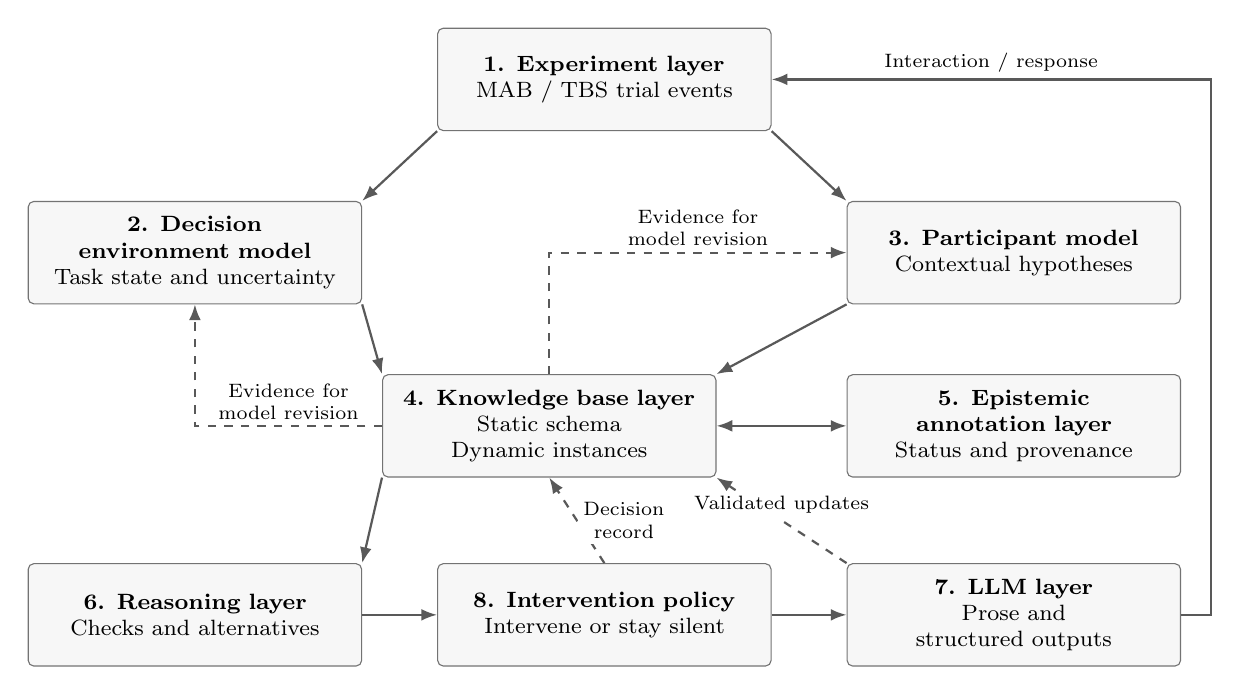
\begin{tikzpicture}[
 box/.style={draw=black!55,rounded corners=2pt,fill=black!3,
   align=center,font=\footnotesize,minimum height=13mm,text width=40mm},
 arr/.style={-{Latex[length=2mm]},thick,draw=black!65},
 record/.style={arr,dashed},
 label/.style={font=\scriptsize,align=center,fill=white,inner sep=2pt}]
\node[box] (experiment) at (0,0)
  {\textbf{1. Experiment layer}\\MAB / TBS trial events};
\node[box] (environment) at (-5.2,-2.2)
  {\textbf{2. Decision\\environment model}\\Task state and uncertainty};
\node[box] (participant) at (5.2,-2.2)
  {\textbf{3. Participant model}\\Contextual hypotheses};
\node[box] (kb) at (-0.7,-4.4)
  {\textbf{4. Knowledge base layer}\\Static schema\\Dynamic instances};
\node[box] (epistemic) at (5.2,-4.4)
  {\textbf{5. Epistemic\\annotation layer}\\Status and provenance};
\node[box] (reason) at (-5.2,-6.8)
  {\textbf{6. Reasoning layer}\\Checks and alternatives};
\node[box] (policy) at (0,-6.8)
  {\textbf{8. Intervention policy}\\Intervene or stay silent};
\node[box] (llm) at (5.2,-6.8)
  {\textbf{7. LLM layer}\\Prose and\\structured outputs};
\draw[arr] (experiment.south west) -- (environment.north east);
\draw[arr] (experiment.south east) -- (participant.north west);
\draw[arr] (environment.south east) -- (kb.north west);
\draw[arr] (participant.south west) -- (kb.north east);
\draw[record] (kb.west) --
  node[label,above]{Evidence for\\model revision} (-5.2,-4.4) -- (environment.south);
\draw[record] (kb.north) -- (-0.7,-2.2) --
  node[label,above]{Evidence for\\model revision} (participant.west);
\draw[thick,draw=black!65,{Latex[length=2mm]}-{Latex[length=2mm]}] (kb.east) -- (epistemic.west);
\draw[arr] (kb.south west) -- (reason.north east);
\draw[arr] (reason.east) -- (policy.west);
\draw[arr] (policy.east) -- (llm.west);
\draw[record] (policy.north) -- node[label,right]{Decision\\record} (kb.south);
\draw[record] (llm.north west) --
  node[label,above]{Validated updates} (kb.south east);
\draw[arr] (llm.east) -- (7.7,-6.8) -- (7.7,0) --
  node[label,above]{Interaction / response} (experiment.east);
\end{tikzpicture}
\caption{Solid arrows show the intervention loop and annotation access; dashed arrows show evidence for model revision, decision records and validated LLM updates. Numbers identify components, not execution order.}
\label{fig:architecture}
\end{figure}

\begin{enumerate}
\item \textbf{Experiment layer.} Runs MAB and TBS, recording trial identifiers, available options, displayed information, choices, response times, outcomes and intervention exposure. Events are aligned with Evaluation, Commitment and Feedback so that support can be offered at predefined moments.
\item \textbf{Decision environment model.} Represents current task state, constraints, estimated volatility, feedback reliability, target gap, remaining trials and uncertainty about the environment. In MAB it maintains uncertain reward-value estimates and evidence of change. In TBS it represents explicit probabilities and gains together with horizon and multiplier rules. Random outcomes are distinguished from unreliable or missing feedback.
\item \textbf{Participant model.} Maintains contextual hypotheses about exploration tendency, switching or persistence, sensitivity to feedback, risk adjustment, response to losses and gains, possible overconfidence, hesitation, constraint neglect and intervention preferences. Each hypothesis has an evidence window, confidence and revision conditions. Slow responses alone do not establish hesitation, nor does persistence establish overconfidence.
\item \textbf{Knowledge base layer.} Provides a human-understandable ontology with a mostly static conceptual schema for the two tasks, and dynamic instances for participants, sessions, trials, claims, uncertainties and interventions. Later prototypes may extend the schema to open-ended domains, but the first milestone should remain bounded.
Queries connect a proposed intervention to its supporting observations and task context.
\item \textbf{Epistemic annotation layer.} Marks claims as known, unknown, assumed, inferred, contested, probable, low-confidence, source-dependent or requiring verification. Annotations also record provenance, time, scope and dependencies. These labels need not be mutually exclusive: an inference can be probable, source-dependent and contested.
\item \textbf{Reasoning layer.} Uses explicit uncertainty modelling, simple probabilistic reasoning and rule-based checks to identify candidate issues and alternatives. Later experiments may evaluate argumentation, fuzzy, paraconsistent or nonmonotonic reasoning where they solve a demonstrated need.
\item \textbf{LLM layer.} Produces conversational interaction, free prose explanations and Socratic questions from the inspected state. Structured outputs or function calls propose machine-checkable updates alongside prose. The backend validates these proposals before committing them; the LLM cannot silently promote its interpretation to an observed fact.
\item \textbf{Intervention policy.} Chooses whether to ask, challenge, warn, explain, compare alternatives, highlight dependencies, request evidence or stay silent. It considers uncertainty in both models, evidence strength, expected usefulness, participant preferences, timing and recent intervention burden. Every decision includes an inspectable rationale.
\end{enumerate}

\textbf{Information boundary.} The experiment runner knows the generative reward schedule, but the MAB teammate must infer volatility from the same feedback available to the participant. Hidden probabilities and actual shift times belong in a separate evaluator store. TBS assistance can use displayed probabilities and published rules, but not future outcomes. This prevents apparent effectiveness from being an artefact of privileged information.

\begin{minipage}{\linewidth}
\textbf{A minimal policy loop.} At each eligible intervention point, the system follows the steps below. The numbers link the flow diagram to the corresponding explanations.

\vspace{4pt}
\begin{minipage}[t]{0.35\linewidth}
\vspace{0pt}
\centering
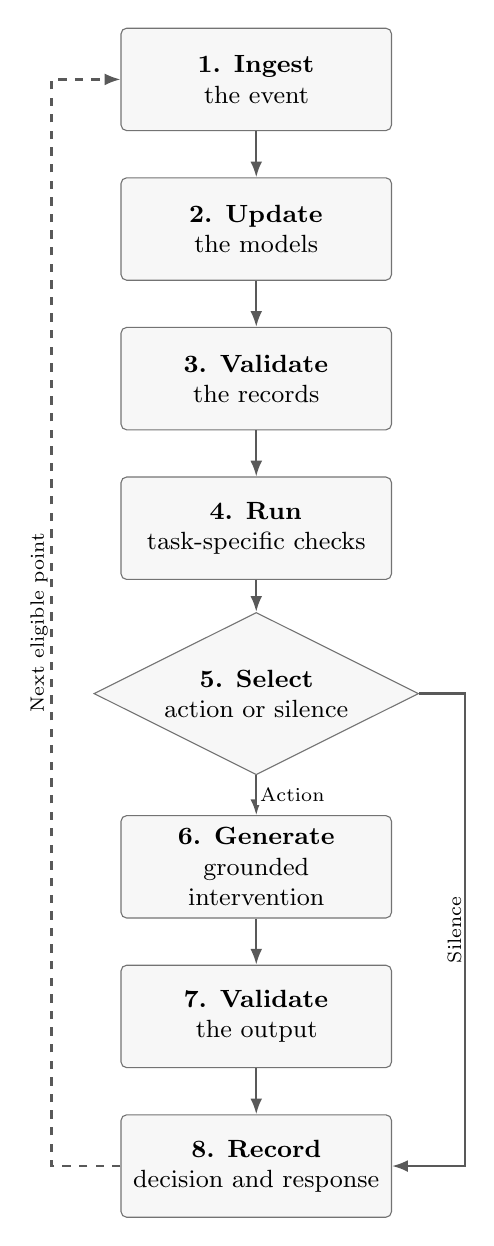
\begin{tikzpicture}[
 flowbox/.style={draw=black!55,rounded corners=2pt,fill=black!3,
   text width=32mm,minimum height=13mm,align=center,font=\small},
 decision/.style={diamond,aspect=2,draw=black!55,fill=black!3,
   text width=27mm,inner sep=1pt,align=center,font=\small},
 arr/.style={-{Latex[length=2mm]},thick,draw=black!65},
 tag/.style={font=\scriptsize,fill=white,inner sep=1pt}]
\node[flowbox] (ingest) at (0,0) {\textbf{1. Ingest}\\the event};
\node[flowbox] (models) at (0,-1.9) {\textbf{2. Update}\\the models};
\node[flowbox] (records) at (0,-3.8) {\textbf{3. Validate}\\the records};
\node[flowbox] (checks) at (0,-5.7) {\textbf{4. Run}\\task-specific checks};
\node[decision] (select) at (0,-7.8) {\textbf{5. Select}\\action or silence};
\node[flowbox] (generate) at (0,-10) {\textbf{6. Generate}\\grounded\\intervention};
\node[flowbox] (validate) at (0,-11.9) {\textbf{7. Validate}\\the output};
\node[flowbox] (record) at (0,-13.8) {\textbf{8. Record}\\decision and response};
\draw[arr] (ingest) -- (models);
\draw[arr] (models) -- (records);
\draw[arr] (records) -- (checks);
\draw[arr] (checks) -- (select);
\draw[arr] (select) -- node[tag,right]{Action} (generate);
\draw[arr] (generate) -- (validate);
\draw[arr] (validate) -- (record);
\draw[arr] (select.east) -- (2.65,-7.8) --
  node[tag,rotate=90,above]{Silence} (2.65,-13.8) -- (record.east);
\draw[arr,dashed] (record.west) -- (-2.6,-13.8) --
  node[tag,rotate=90,above]{Next eligible point} (-2.6,0) -- (ingest.west);
\end{tikzpicture}
\end{minipage}\hfill
\begin{minipage}[t]{0.61\linewidth}
\vspace{0pt}
\small\raggedright
\setlength{\parskip}{1pt}
\begin{enumerate}[leftmargin=1.4em,itemsep=3pt,topsep=0pt]
\item \textbf{Ingest the event.} The experiment layer records the current trial event and the information available to the participant.\par\emph{Module: Experiment layer.}
\item \textbf{Update the models.} Revise environment estimates and contextual participant hypotheses, retaining uncertainty and competing interpretations.\par\emph{Module: Decision environment and participant models.}
\item \textbf{Validate the records.} Check the proposed knowledge-base updates and their epistemic annotations before committing them.\par\emph{Module: Knowledge base and epistemic annotation layers (backend validator).}
\item \textbf{Run task-specific checks.} The reasoning layer identifies candidate issues, relevant evidence and plausible alternatives.\par\emph{Module: Reasoning layer.}
\item \textbf{Select an action or silence.} The intervention policy ranks candidates by evidential support, decision relevance and interruption cost; it selects silence if none clears the current threshold. Initial thresholds and cooldowns should be explicit, preregistered parameters, not implied optimal values. Silence bypasses message generation and output validation but is still recorded.\par\emph{Module: Intervention policy.}
\item \textbf{Generate a grounded intervention.} If intervention is selected, the LLM expresses the chosen action using the supporting claim and permitted task information.\par\emph{Module: LLM layer.}
\item \textbf{Validate the output.} Check the proposed message and structured updates for consistency with the selected action, available evidence and output schemas before delivery or commitment. A generated message is delivered only after validation.\par\emph{Module: Backend validator, using reasoning-layer and intervention-policy checks.}
\item \textbf{Record the decision and response.} Store the policy rationale, including reasons for silence, any delivered message and any subsequent participant response for inspection and replay.\par\emph{Module: Knowledge base and experiment layers.}
\end{enumerate}
\end{minipage}
\end{minipage}

\section{A static schema and dynamic instances}
For the first prototype, the two well-defined experiments permit specifying alternatives, feedback mechanisms, target conditions and decision horizons in advance, so the prototype needs not invent new concepts to interpret each trial. Therefore, we can have \emph{a static schema} and \emph{dynamic instances}:  
\begin{itemize}
  \item \textbf{Static schema.} A fixed ontology defines the types of entities and relationships that can be represented, including environments, events, task-state variables, participant patterns, claims, epistemic statuses and intervention types. Relations such as \texttt{observedIn}, \texttt{supportedBy}, \texttt{dependsOn}, \texttt{contradicts} and \texttt{revises} connect them. A versioned schema can be revised between experiments, while remaining fixed within a study.
  \item \textbf{Dynamic instances.} Each participant session generates a set of instances that capture the unfolding of the environment, participant behavior and session events. These instances include trial events, inferred patterns, unresolved uncertainties and intervention records.
\end{itemize}

The closed schema is a deliberate experimental foundation for the longer-term ambition of creating a general AI teammate capable of open-ended modelling across unfamiliar decision situations. In those settings, we may not assume that all relevant goals, actors, constraints, evidence types or relationships have been anticipated. The teammate must recognise when its existing vocabulary is inadequate, propose new concepts or distinctions, and reconsider how earlier observations should be represented. Productive ignorance must then concern both uncertainty \emph{within} a model and uncertainty about the model's \emph{adequacy}: an omitted dependency or an inappropriate category may matter as much as an unknown parameter.% Extending the ontology should preserve provenance and unresolved disagreement, with human-reviewed revisions rather than silent changes to the meaning of existing claims.

\section{Personalization}
Personalised support lives in the participant model, linked to the environment model and knowledge base. The question is ``How is this person deciding in this situation?'' rather than ``What kind of decision-maker is this person?'' A tendency observed in volatile learning should not transfer automatically to a task with explicit probabilities and changing targets. 

Personalization is implemented across several components, not confined to a single module. The participant model maintains hypotheses about the person's decision patterns, while the environment model captures the current task state and its uncertainty. The knowledge base and epistemic annotations preserve these hypotheses, their supporting evidence and their uncertainty. The reasoning layer identifies relevant issues, the intervention policy decides whether and how to intervene, and the LLM layer expresses the selected intervention.

The participant model must be \emph{inspectable, revisable and humble}. It must be possible to inspect the observations behind a hypothesis, its uncertainty, competing explanations and what would count against it. Evidence can expire or lose relevance after an environmental change. Participant corrections become attributed evidence rather than unquestionable truth. Overconfidence requires a mismatch between elicited confidence and an appropriate evidential benchmark; behavior alone is insufficient.

Personalisation should depend jointly on what the teammate learns about the participant and the current decision context. As evidence accumulates about volatility, feedback reliability, target gap and remaining opportunities, it can revise the timing, frequency, phrasing and intensity of support. For example, evidence of a possible volatility shift may justify asking a persistent participant what would warrant renewed exploration; as a target-based horizon contracts, support may focus on whether the current strategy can still reach the target. If the contextual interpretation remains weak or contested, the teammate should use a tentative question or remain silent. Participant preferences should be elicited and updated from feedback, but interpreted alongside these changing demands. A preference for infrequent prompts may favour waiting for a sustained pattern, while evidence that delay would make a question less useful may warrant an earlier, brief intervention. Effectiveness should be assessed independently of satisfaction or compliance.

\section{Development roadmap}
The preceding sections describe the design for Phase~1 of a larger research plan. Phases~2 and~3 extend this foundation towards professional scenarios and, ultimately, an open-ended AI teammate.

\begin{enumerate}
\item \textbf{Phase 1: Closed ontology, controlled tasks.} Implement the two task environments, fixed schema, trial logging, simple uncertain models and a small library of intervention rules. Deliver replayable traces, schema validation and the four-condition pilot. The bounded ontology is a strength: it makes information access, model errors and intervention consequences experimentally controllable.
\item \textbf{Phase 2: Semi-open ontology, professional scenarios.} Extend to selected scenarios with domain experts. Retain a stable core but allow reviewed additions for goals, constraints, evidence and conflicting interpretations. Test transfer, workload and whether participant hypotheses remain valid across contexts; do not infer professional effectiveness from game performance.
\item \textbf{Phase 3: Open Socratic teammate with human-reviewed ontology revision.} Allow proposed concepts and relations from novel situations, with explicit provenance, versioning and human review before adoption. Evaluate semantic drift, unresolved disagreement and the teammate's ability to justify its intervention authority in less structured collaboration.
\end{enumerate}
%Progression should depend on demonstrated grounding, judgment benefits and tolerable intervention cost, rather than conversational fluency alone.

\section{Candidate technology stack}
The larger research programme calls for a modular stack that can grow from controlled experiments to professional scenarios and an open-ended teammate. Its main capabilities are experimental interaction, inspectable knowledge representation, uncertainty modelling, validation, conversational delivery and coordination of the intervention loop. The following technologies are candidates for these roles; they are alternatives and possible extensions, rather than a single configuration that must be implemented in full.
\begin{itemize}
\item \textbf{Experiments and interaction:} whatever implementation already exists for the MAB and TBS tasks.
\item \textbf{Backend:} Python/FastAPI for event ingestion, state updates, model services and a versioned intervention API.
\item \textbf{Ontology and knowledge base:} Prot\'eg\'e/WebProt\'eg\'e for ontology design; RDF/OWL/SPARQL with RDFLib or Owlready2 for implementation. RDFLib provides Python graph handling and SPARQL support.\footnote{\url{https://rdflib.readthedocs.io/en/stable/}} Apache Jena/Fuseki could support a shared graph store or endpoint if later phases require one.
\item \textbf{Validation:} SHACL/pySHACL for claim shapes, evidence links and required metadata, alongside checks of LLM output schemas and task-rule consistency.

%RDF/OWL supplies structure and relationships; calibrated uncertainty and the treatment of contradictory assertions require explicit modelling and application rules. For Phase~1, contested propositions should remain annotated claim objects, with unknown distinguished from false. SHACL checks record structure, while the model and policy code determine how uncertainty affects intervention. This division makes productive ignorance inspectable and experimentally testable within the bounded prototype.

\item \textbf{Probabilistic modelling:} pgmpy for the initial Bayesian-network runtime model, followed by PyMC for empirical estimation and analysis, with complexity guided by evidence and calibration results.
\item \textbf{Argumentation:} a simple Python module for supporting and opposing reasons; possible later evaluation of TweetyProject or Carneades as requirements for defeasible reasoning become clearer.
\item \textbf{Language and orchestration:} an LLM API with structured outputs/function calling; LangGraph or similar orchestration if the workflow grows to require persistent state, multiple reasoning steps and human review checkpoints.\footnote{\url{https://docs.langchain.com/oss/python/langgraph/overview}}
\end{itemize}

The following subsections the validation, probabilistic modelling and argumentation components, which are central to productive ignorance and the Socratic intervention loop.

\subsection{Knowledge-base validation with SHACL/pySHACL}
SHACL (Shapes Constraint Language) specifies conditions that an RDF data graph must satisfy.\footnote{\url{https://www.w3.org/TR/shacl/}} Whereas the ontology defines concepts and relationships, SHACL \emph{shapes} specify what constitutes an acceptable record: required properties, permitted values, datatypes, cardinalities and links to entities of the appropriate type. pySHACL is a Python implementation that checks the data against these shapes and returns a conformance result and validation report.\footnote{\url{https://github.com/RDFLib/pySHACL}} It therefore provides an explicit validation layer for the dynamic instances created during a session.

For Phase~1, a small set of hand-written shapes should cover trials, participant hypotheses, epistemic annotations and intervention records. A trial should identify its participant, session and trial index. An inferred participant hypothesis should identify its task context, supporting evidence, epistemic status and model version; a numerical confidence, when present, should lie between zero and one and specify its interpretation. An intervention record should identify the selected action, its rationale and supporting claims, including an explicit rationale when the action is silence. These requirements make missing evidence or metadata visible before the record informs further reasoning.

In the minimal policy loop, pySHACL belongs primarily to step~3, which validates proposed knowledge-base updates before commitment. The backend should validate a candidate graph containing the proposed records and their relevant context, retain the report, and reject or return invalid updates for correction. Structured LLM proposals should first pass their output-schema checks; any resulting RDF updates should then pass the relevant shapes before entering the knowledge base. For example, a hypothesis of premature exploitation without a supporting trial link should fail its shape, even if the LLM's prose sounds plausible.

Conformance establishes that a record meets the declared constraints, not that its claim is true, its probability is calibrated or an intervention is justified. SHACL should permit unknown and contested claims when their epistemic status and provenance are properly recorded. Probabilistic inference, policy checks and output validation remain responsible for evidential interpretation, intervention selection and message consistency. Together, these mechanisms preserve uncertainty while enforcing a traceable, machine-checkable record of what the teammate believes and does.

\subsection{Probabilistic modelling: runtime inference and empirical refinement}
The first prototype should use pgmpy for a small, transparent Bayesian-network runtime model.\footnote{\url{https://pgmpy.org/examples/Inference_Discrete_BN.html}} This is appropriate because MAB and TBS are controlled, well-defined environments whose task variables and dependencies can be specified in advance. The initial network should be hand-designed from task structure and theory, with explicit, provisional conditional probability tables, rather than blindly learned from a small dataset. Its assumptions should be documented and checked for sensitivity.

The network should use discrete, interpretable states: low/medium/high volatility evidence, low/high switching, and hypotheses such as underexploration, premature exploitation, constraint neglect and feedback overweighting. A further variable can represent likely intervention usefulness, conditional on the task context, participant hypotheses and candidate intervention. During the task, pgmpy should support real-time inference to help the policy decide whether to ask, challenge, warn, explain, highlight a dependency or stay silent. An illustrative runtime query is:
\begin{quote}\small\ttfamily
P(premature\_exploitation | volatility\_shift,\\
\hspace*{1em}low\_switching, declining\_expected\_value)
\end{quote}
Here, volatility shift denotes evidence of a suspected change, and declining expected value is inferred from permitted feedback; neither supplies privileged access to hidden task state.

The outputs should remain inspectable and linked to ontology instances and the participant model. Each inferred participant-state hypothesis should retain its input evidence, posterior estimate, model version and relevant assumptions. The policy should separately record how that inference, estimated intervention usefulness and interruption cost led to a chosen or withheld intervention. A posterior supports deliberation by the policy; it does not establish a diagnosis or automatically justify a prompt.

PyMC should be introduced in a second stage, once trial-level data have been collected, for richer statistical modelling and analysis. Hierarchical Bayesian models can represent participant behaviour, individual differences, environment-specific effects and uncertainty around intervention effects.\footnote{\url{https://www.pymc.io/projects/examples/en/2022.01.0/case_studies/multilevel_modeling.html}} A concrete goal is to estimate participant-specific adaptation rates and responsiveness to Socratic intervention, with partial pooling across participants and explicit differences between MAB and TBS. This analytical stage can begin within Phase~1; it is distinct from the roadmap's expansion to professional scenarios in Phase~2.

PyMC need not replace pgmpy. Empirical estimates can refine the runtime model's priors, transition probabilities, policy thresholds and intervention-effect assumptions, with uncertainty retained and revisions evaluated before deployment. The division of labour is: \emph{``pgmpy helps build the first Socratic teammate; PyMC helps learn whether and why it works.''}


\subsection{Argumentation: supporting, opposing and revisable reasons}
An argumentation module should expose the reasons for and against a participant-state hypothesis or candidate intervention. The Bayesian network estimates uncertainty; argumentation records how premises support a conclusion, which objections challenge it, and what would warrant revision. The reasoning is \emph{defeasible}: new evidence or an exception can overturn a previously supported conclusion. Productive ignorance therefore includes preserving unresolved objections alongside the current interpretation.

For Phase~1, a simple Python module should suffice. Each argument should record its conclusion, premises, supporting trial or claim identifiers, scope and epistemic status, with links to opposing reasons or challenged assumptions. Hand-written rules can construct these records from the ontology, participant model and probabilistic outputs. Explicit evaluation rules should distinguish supported, opposed and unresolved candidates and retain their rationale. Posterior estimates may inform premises, but argument strength should not automatically be treated as a calibrated probability. The module contributes to step~4 of the minimal policy loop; step~5 decides whether the resulting case justifies intervention.

In MAB, declining reward estimates and persistent choice after a suspected shift may support asking about renewed exploration. Noisy feedback may challenge the shift interpretation, and a recent prompt may count against intervening now. Preserving these objections can justify a tentative question or silence. In TBS, a large target gap and few remaining choices may support reviewing the strategy, while the final-trial multiplier may undermine the assumption that the target is unreachable. The LLM should express the inspected reasons and unresolved assumptions; the intervention record should retain the arguments used by the policy.

A fuller framework becomes relevant when professional scenarios introduce interacting exceptions, chains of objections or competing standards for accepting claims. TweetyProject offers argumentation and defeasible-reasoning libraries,\footnote{\url{https://tweetyproject.org/}} while Carneades provides tools for argument reconstruction, evaluation and mapping.\footnote{\url{https://carneades.github.io/}} Either should be evaluated against concrete requirements for inspectability, unresolved conflict, runtime integration and reproducibility. The first prototype should test whether explicit supporting and opposing reasons improve intervention decisions before adopting a more elaborate engine.

\section{Closing research claim}

\textbf{The first prototype tests whether productive ignorance can be operationalized in controlled decision environments through a fixed ontology, dynamic epistemic annotations, participant modelling, and adaptive Socratic intervention.}
\end{document}
